\chapter{E-commerce background} \label{chap:ecommerce}

\section*{}

% Neste capítulo é descrito o estado da arte e são
%apresentados trabalhos relacionados para mostrar o que existe no
%mesmo domínio e quais os problemas em aberto.
%Deve deixar claro que existe uma oportunidade de desenvolvimento que
%cobre alguma falha concreta .

%O capítulo deve também efetuar uma revisão tecnológica às principais
%ferramentas utilizáveis no âmbito do projeto, justificando futuras
%escolhas.

In this chapter we discuss some key concepts related to e-commerce, for the 
purpose of giving context to the dissertation. We discuss the typical customer 
life cycle in an e-commerce website, some metrics that might be used and some 
ways on how the customer interaction with the website might be influenced and 
improved.

\section{Introduction}

E-commerce, or electronic commerce, can be described by the trading of products 
or services over the Internet (or other computer networks). The type of 
e-commerce businesses we are interested are those who sell their goods directly 
to the customer, e.g online shopping, using an online store or catalog of 
products. Some popular online 
stores\footnote{\url{http://www.alexa.com/topsites/category/Top/Shopping}} are 
Amazon\footnote{\url{http://www.amazon.com/}}, 
Ebay\footnote{\url{http://www.ebay.com/}} and 
Alibaba\footnote{\url{http://www.alibaba.com/}}.

\section{Customer life cycle}

An important concept to understand the customer is by describing its life 
cycle, as presented by~\cite[Section 6]{Sterne2000} in 
figure~\ref{fig:lifecycle}.

\begin{figure}[h]
  \begin{center}
    \leavevmode
    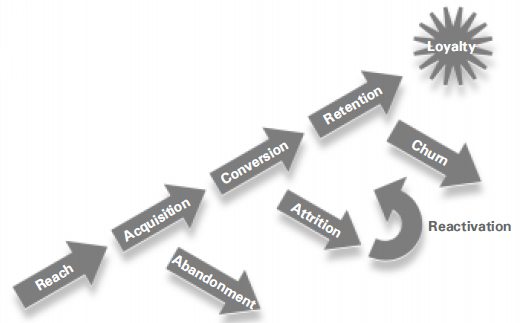
\includegraphics[width=0.86\textwidth]{lifecycle}
    \caption{Customer lifecycle \cite{Sterne2000}}
    \label{fig:lifecycle}
  \end{center}
\end{figure}

It starts by reaching the target audience or market up to an established 
customer base, not forgetting about those that drop mid way, due to abandonment 
or attrition.

\begin{itemize}
    \item Reach happens outside of the website and refers to the number of 
    potential customers. For example, if the online store is advertised on a 
    social network, the reach is the number of users who were served the ad in 
    that other website, they may or may not ignore it.
    \item Acquisition is the next stage, where the user decides to act on and 
    visits the website (or some other action like subscribing to a newsletter).
    \item Conversion is the stage where a visitor stops being a user and starts 
    being a customer. It usually means that the user made a purchase but some 
    companies might consider a sign up or registration in the website as a 
    conversion.
    \item Retention focuses on making existing customers, that made at least 
    one purchase before, repeat purchases.
    \item Loyalty is a strong form of retention, which represents a greater 
    trust level of the customer in the store.
    \item Abandonment is defined by the customers that started the buying 
    process but do not finish it. For example, a customer may add items to the 
    online shopping cart but instead of moving to the next step, e.g. enter 
    credit card details, they exit the website or go elsewhere. This may happen 
    in any store with a multi-step buying process, which is very common.
    \item Attrition happens when a retained customer ceases buying from the 
    store and starts using a competitor store.
    \item Churn is defined by the number of customer that attrited during a 
    certain period divided by the total number of customers at the end of that 
    period. It measures how much of the customer base "rolls over" in a certain 
    time period.
\end{itemize}

\section{Customer Behavior Model Graph (CBMG)}



\section{E-commerce metrics}

\cite{Sterne2000}

\section{Influencing user behaviour}

-> influenciar behaviour em vez de recom

\subsection{Recommendation engines}

\cite{Adomavicius2005}

\section{Summary}

No final do capítulo deverá ser apresentado um resumo com as 
principais conclusões que se podem tirar. 
